\section{Use Cases and Numerical Experiments}
\label{chap:useCases}
<<<<<<< HEAD
In this section, we describe the use cases which were used to proof that our approach for the automatic opitimized creation of railway timetables performes. 

\begin{itemize}
	\item[1)] Anwering a short-term train path request within three minutes
	\item[2)] Creating a timetable for one day 
\end{itemize}
=======
In this section, we describe two use cases (Section~\ref{chap:CnR} and~\ref{chap:Netzfahrplan}) to which we are able to apply the methods mentioned before. For each use case we provide numerical experiments showing the threefold benefit of faster response times, increased capacity usage and reduced travel times.
>>>>>>> e526041c494212ee1d2b8d7f41bb0804cf9acc09

\subsection{Click \& Ride App}
\label{chap:CnR}
For a short-term train path request, e.g.\ a train run for the next day, we can improve the response time to the railway operator by using our approach in a fully automated process. We will introduce the new way of booking a train path with a mobile application called \emph{Click\&Ride-App}. We commit to get the railway operator a train path offering within no longer than three minutes. In comparison, today's process for manual planning takes several hours or even up to three days. To ensure a maximum duration of three minutes we need to automate every single step in the planning process. A simplified process sequence is shown in Figure~\ref{fig:process_sequence}.
%
\begin{figure}[htb]
	\centering
	% If you include a JPG file,
	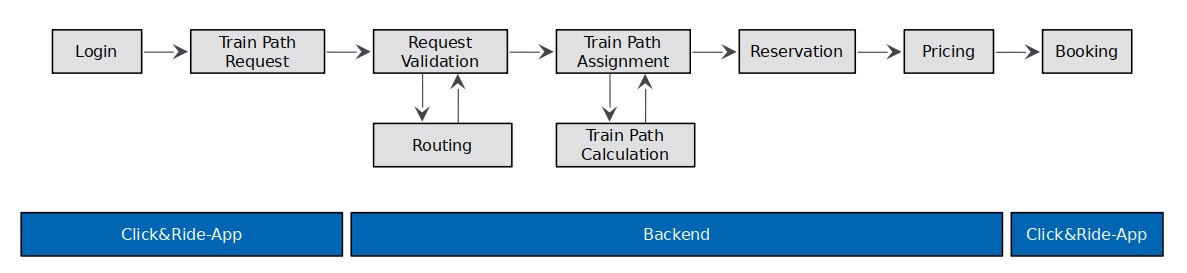
\includegraphics[width=\textwidth]{Bilder/process_sequence.jpg}
	% Else if you include an EPS file
	%    (it may need an interpreter for the PostScript language, e.g. Ghostscript),
	%\includegraphics[scale=0.30]{Fig1_Track.eps}
	\caption{Simplified process of Click\&Ride. The process is fully automated except for login and requesting a train path as well as booking.}
	\label{fig:process_sequence}
\end{figure}

Click\&Ride is a new B2B channel so only railway operators may use the functionalities. After logging in, the the train path request will be submitted to the back-end processes. At first there is a validation service that ensures formal and technical fit to the lines that will be used. For example an electric vehicle cannot use a line with no overhead line. If there are any problems with the train path request the railway operator gets instant feedback on the app's screen and can fix the problem. When there are no problems left the train path request is handled by the optimization in train path assignment (see Section~\ref{chap:Belegung}). If the technical properties of the requested train do not match the existing slots on the lines, a train path is generated automatically by train path planning as described in Section~\ref{chap:Konstruktion}. Railway operators have a limited time to check the offered train path before booking. To make sure the capacity on the line cannot be given to other railway operators in the meanwhile, the train path is reserved for a maximum of ten minutes. To complete the response the total price for the train path is calculated and displayed in the Click\&Ride-App. An example response is shown in Figure~\ref{fig:CnR_response}.
\begin{figure}[htb]
	\centering
	% If you include a JPG file,
	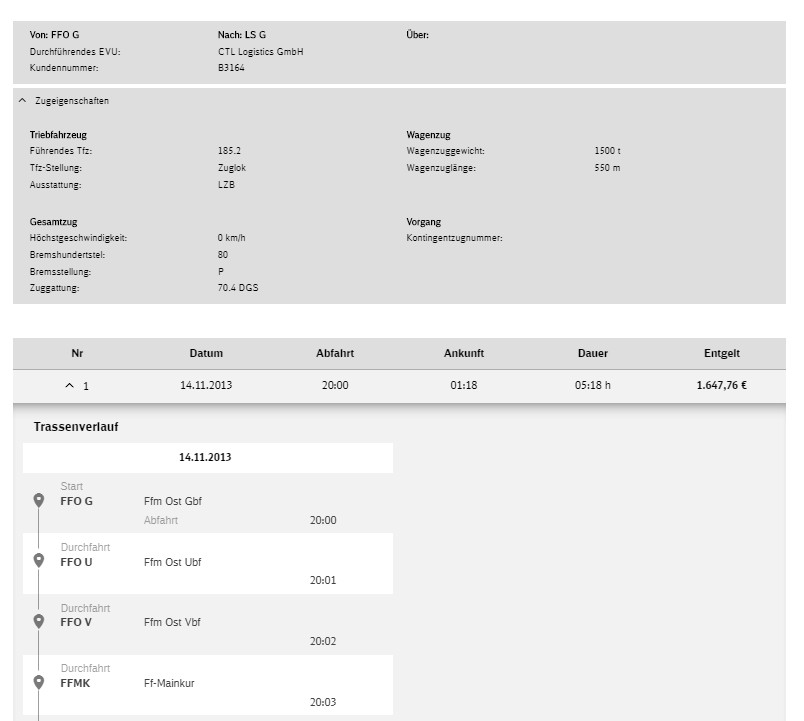
\includegraphics[width=\textwidth]{Bilder/train_path.jpg}
	% Else if you include an EPS file
	%    (it may need an interpreter for the PostScript language, e.g. Ghostscript),
	%\includegraphics[scale=0.30]{Fig1_Track.eps}
	\caption{Example Train Path in Click\&Ride}
	\label{fig:CnR_response}
\end{figure}

\subsubsection{Numerical Experiments}
For our experiments we use $1182$ real customer requests, which were put on November, 14th, 2013 in Germany. In doing so, a customer request consists of the running points, time requirements and the characteristics of the train. The running points are at least the start of the request and its goal, but may also include some stops which should be served in between. The time requirements for our data consists only of an interval at the start of the request. But it is also possible to provide further time restrictions on the other running points. The characteristics of the request include all data necessary to calculate its dynamic properties such as acceleration and its static parameters like length, width and mass of the requested train. Consequently, we consider the infrastructure available in 2013. Furthermore, we also regard the blockages of passenger trains, which were scheduled on November, 14th, 2013 in order to have a realistic setup.
%
\begin{table}[h]
	\centering
	\caption{Response times in seconds for $1182$ requests provided in percentiles.}
	\label{tab:result_CnR}
	\begin{tabular}{ccccc} \hline
		$\textbf{50\%}$ & $\textbf{90\%}$ & $\textbf{95\%}$ & $\textbf{99\%}$ \\ \hline
		$8.47$ sec.     & $66.74$ sec.    & $138.30$ sec.   & $216.55$ sec.   \\
	\end{tabular}
\end{table}
\par

The experiments, as provided in Table~\ref{tab:result_CnR}, show that $95\%$ of the request are served within $138.30$ seconds and the maximal response time is $431.10$ seconds. This is a vast improvement compared to the up to three days required in the current manual process.

\subsection{Netzfahrplan}
\label{chap:Netzfahrplan}
<<<<<<< HEAD
To create an automatic timetable for one day first you need to calculate the slots, where each slot starts and ends in one Betriebsstelle. Also every slot has up to three different train charakteristics and an amount of how many slots of which charakteristic are supposed to be produced. Those infomartion are necessary to preproduce a optimal set of slots with their most variety for the trainpath assignement.  \\
The second step is the train path assignment which needs the customer request. A customer request consist of the running points, time requirements and the characteristics of the train. The running points are at least the start of the request and its goal, but may also include some stops which should be served in between. The time requirements for our data consists only of an interval at the start of the request. But it is also possible to provide further time restrictions on the other running points. The characteristics of the request include all data necessary to calculate its dynamic properties such as acceleration and its static parameters like length, width and mass of the requested train.  \\
To discuss the solution of our process we created the slots for the european rail freight corridor one. Corridor one is the Rhine-Alpine Corridor stretches from sea ports of Rotterdam, Zeebrugge, Antwerp, Amsterdam and Vlissingen to the port of Genoa. During the course it passes five different countrys: Netherlands, Belgium, Germany, Switzerland and Italy. Here only the part in Germany Emmerich/Aachen to Basel will be considered. (see picture XXX). \\


=======
The introduced methods also allow to change the process of the \emph{Netzfahrplan}, which is the process of creating a timetable for a whole year. In this use case all customer requests, for passenger and freight trains, are put at the same time and have to be provided with a timetable fulfilling all requests within $40$ days. This means a huge effort to DB Netz and can be eased b< planing the freigth trains automatically In an iterative process we manually create timetables for the passenger trains first. In the second step, the freight trains are calculated automatically with the methods described in Sections~\ref{chap:Konstruktion} and~\ref{chap:Belegung}. After that, the timetables are adapted and improved, iteratively.

\textbf{\textcolor{red}{Falls noch Platz, könnte hier das Schaubild hinzufügen}}

\subsubsection{Numerical Experiments}
For this experiment we also consider the data from NOvember, 14th, 2013 regarding infrastructure, blockages and customer requests For clarity of presentation we restrict the shown results to the Korridor 1 \cite{} rather than Germany. That means, we only consider requests and infrastructure of that specific part of Germany. Thus, we have a test consisting of $\textbf{\textcolor{red}{??}}$ requests and create slots on $\textbf{\textcolor{red}{??}}$ sections (compare Figure~\ref{}).

FIGURE / TABLE RESULTS

Table/Figure shows that we increase the number ... DISCUSS RESULTS
>>>>>>> e526041c494212ee1d2b8d7f41bb0804cf9acc09
%
\begin{table}[h]
	\centering
	\caption{Results for Netzfahrplan}
	\label{tab:result_Netzfpl}
	\begin{tabular}{lcccc} \hline
		\textbf{Text Style}   & \textbf{Font} & \textbf{Style} & \textbf{Size (pt)} \\ \hline
		Main text             & Times         & regular        & 10                 \\
		Section heading       & Times         & bold           & 12                 \\
		Subsection heading    & Times         & bold           & 10                 \\
		Subsubsection heading & Times         & bold           & 10                 \\ \hline
	\end{tabular}
\end{table}
\par


